\chapter{Design}

% Software Requirements
% Hardware Requirements
% Software Requirements Specification
	% Functionality
		% What is the software supposed to do?
	% External Interface
		% How does the software interact with people, the system's hardware, other hardware, and other software?
		% What assumptions can be made about these external entities?
	% Required Performance
		% What is the speed, availability, response time, recovery time of various software functions and so on?
	% Quality Attributes
		% What are the portability, correctness, maintainability, security, and other considerations?
	% Design Constraints imposed on an implementation
		% Are there any required standards in effect, implementation language, policies for database integrity, resource limits, operating environment(s) and so on?

\section{Software Requirements}
\paragraph{}
For the PC (LaaS server):
\begin{enumerate}
\item Any operating system with a Python interpreter available
\item Python 2.7
\item Flask micro-framework for implementing web service (package ``flask")
\item SciKit Learn ML library for Python (package ``sklearn")
\end{enumerate}

\paragraph{}
For the Raspberry Pi (device controller):
\begin{enumerate}
\item Raspbian OS for the Pi
\item Python 2.7
\item Flask micro-framework for implementing controller's web interface (package ``flask")
\end{enumerate}

\section{Hardware Requirements}

\begin{enumerate}
\item A personal computer
\item A Raspberry Pi Single Board Computer (SBC)
\item Proper network infrastructure
\end{enumerate}

\pagebreak

\section{Software Requirements Specification}

\subsection{Functionality}
\paragraph{}
We intend the software to be divided over two tiers: the interface and the LaaS Server. The user is served up a web interface to the smart devices connected to the Raspberry Pi over a conventional TCP/IP network. It will be possible to view the states of individual devices and change them. Such usage of the system can happen even in the absence of the Machine Learning Service. That is to say, the first tier consists of an independent interfacing system that enables the user to control connected smart devices, and this may optionally utilize a usage-prediction-oriented machine learning service if it is available.
\paragraph{}
The second tier consists of a special case of SaaS (Software-as-a-Service), called LaaS (Learning-as-a-Service). This service is intended to provide proper WebAPI for the tier one application to communicate with. Data can be sent by the tier one application to the LaaS service using this API, which will then be processed continuously to generate predictions for individual devices. These predictions can also be requested by the tier one application so it can apply it in real-time to the smart environment it is providing an interface to. Non-availability of the services in this tier will not affect the user interfacing system implemented in the first tier, except for the unavailability of predictions.
\paragraph{}
Unavailability of the first tier, id est interface tier, is fatally deteriorating to the user experience. This tier must always be available and smoothly working, that is to say, it should be robust. The second tier provides a service which is not necessarily central to  the functioning of the smart home by design. This means that unavailability of the service will not affect the core control system provided by the first tier.

\pagebreak
\subsection{External Interfaces}
\paragraph{}
Interfacing between different components of this system is crucial to it's execution. We will use conventional communication mechanisms like RESTful WebAPIs for communication between both the client \& first tier, and the first \& second tier.
\begin{figure}[H]
		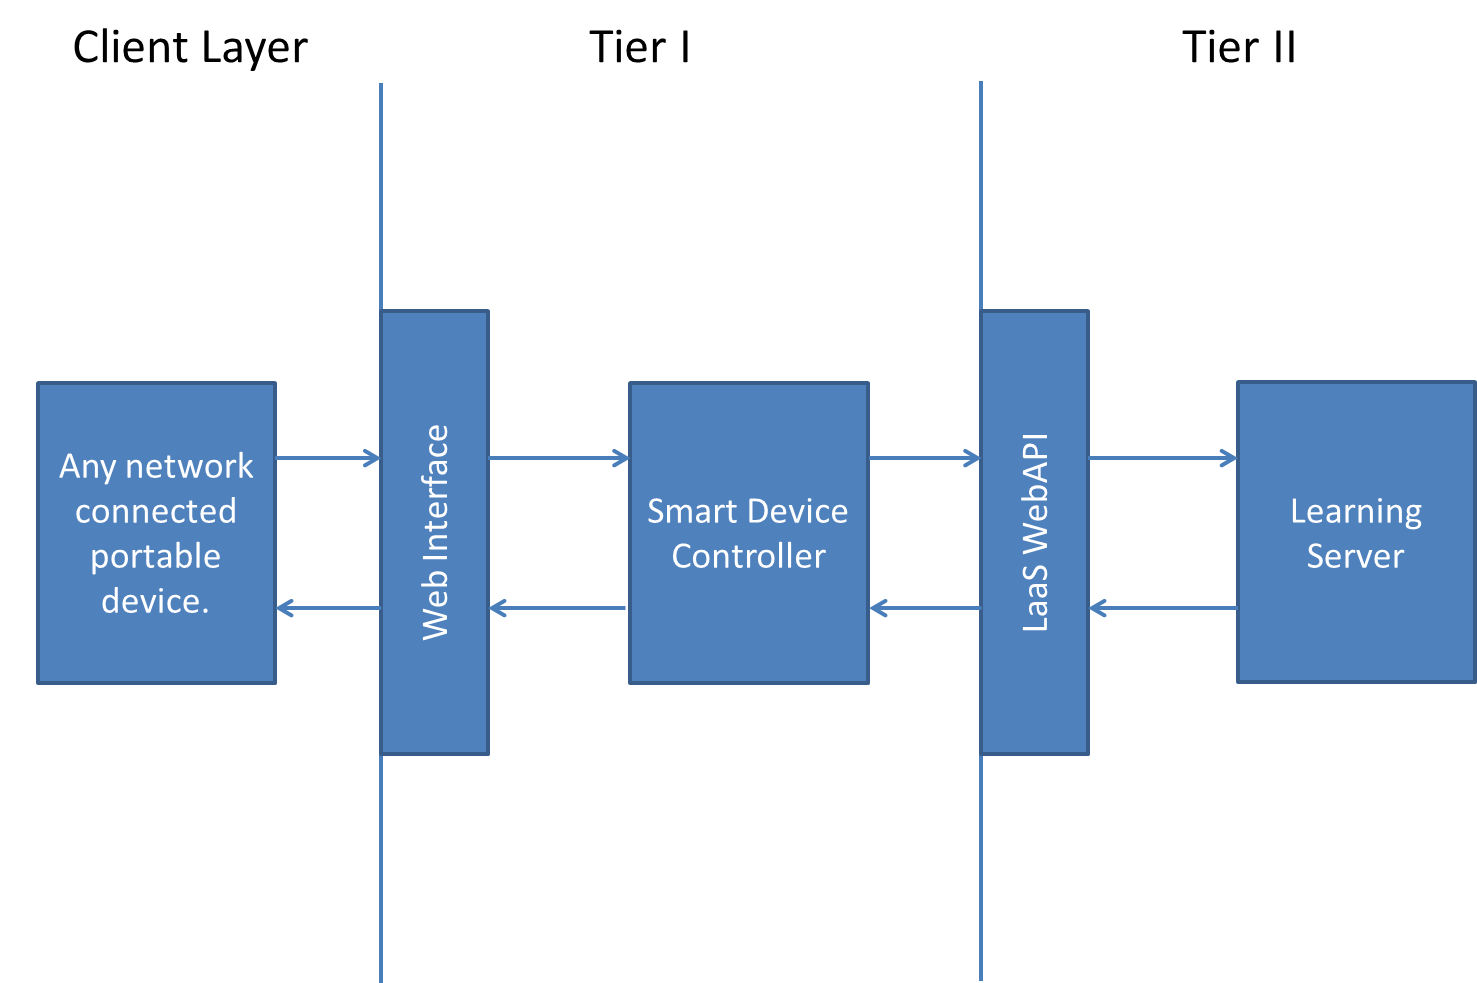
\includegraphics[width=\textwidth]{./Chapter3/client-t1-t2}
			\caption{Overview of Tiered Components and their Interfacing}
	\end{figure}
	\subsubsection*{Client - Tier I Interface}
	\paragraph{}
	The smart environment can be controlled via a web app. This app can be accessed by the user by connecting to the smart devices' controller (the Raspberry Pi) on the standard HTTP Port (port 80). The user can then view current states of the connected smart devices and change them according to their preference.
	\begin{figure}[H]
		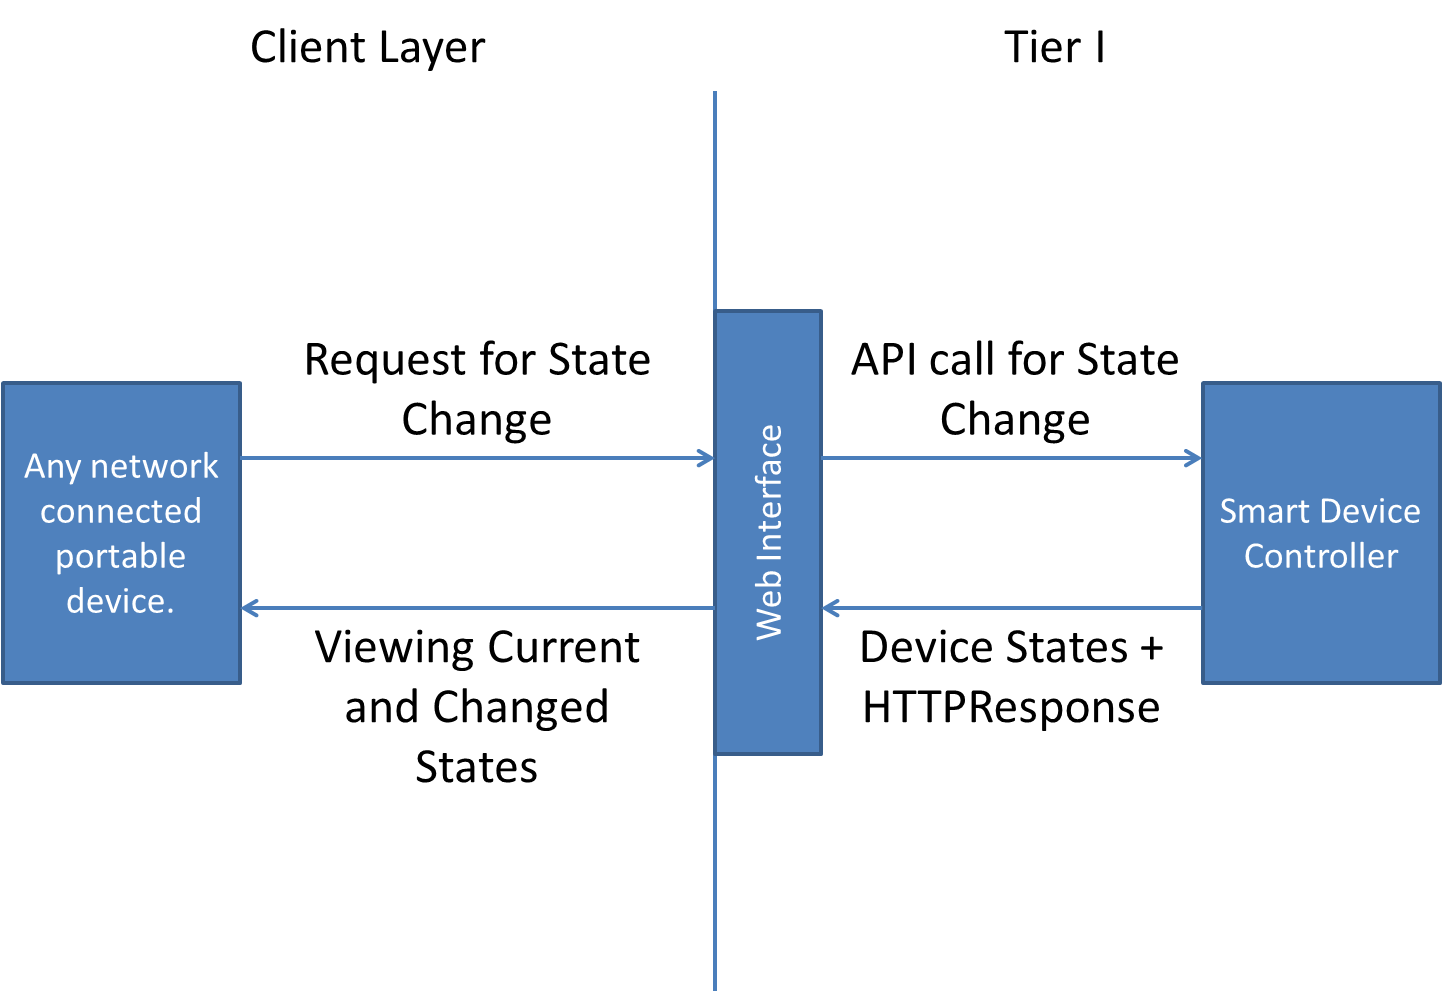
\includegraphics[width=\textwidth]{./Chapter3/client-t1}
			\caption{Interface between Client and Tier I}
	\end{figure}
	\paragraph{}
	Besides collecting user generated actions, the controller may also collect external data (like current weather) in order to facilitate prediction of user actions based on regressive correlation with external influncers.
	\paragraph{}
	This interface is critical as it delivers the frontend for our system to the user. Network delay or inconsistencies within its implementation directly and drastically affect user experience.
	
	\subsubsection*{Tier I - Tier II Interface}
	\paragraph{}
	The LaaS server can be accessed by the Tier I application through a RESTful WebAPI. The API includes calls for collecting device state changes made by the user and for requesting the prediction based on recent usage data.
	\begin{figure}[H]
		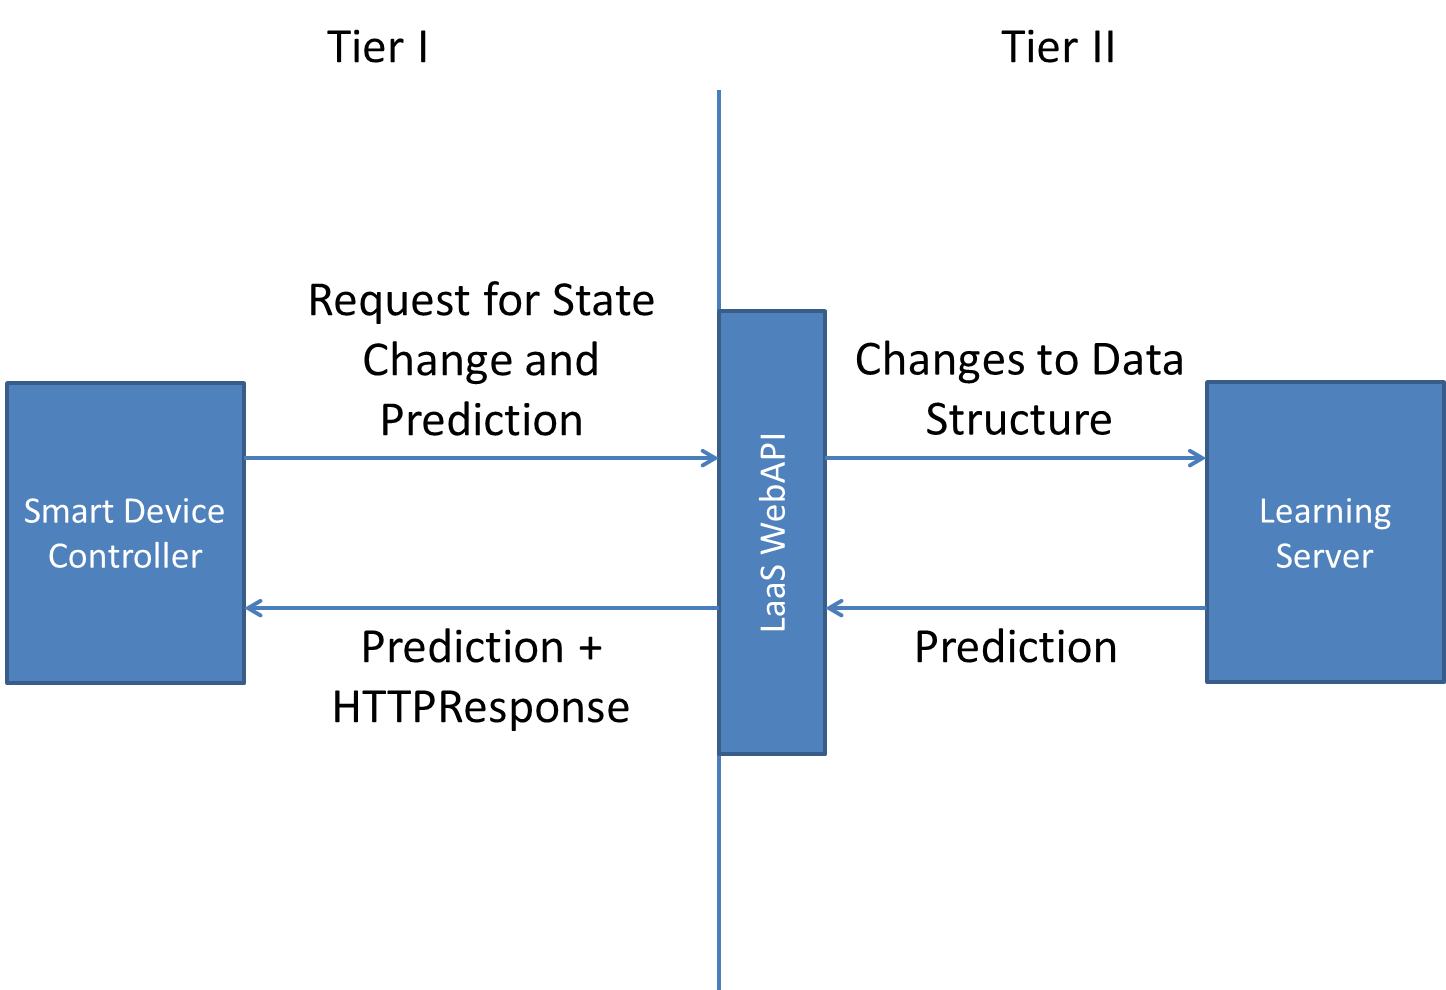
\includegraphics[width=\textwidth]{./Chapter3/t1-t2}
			\caption{Interface between Tier I and Tier II}
	\end{figure}
	\paragraph{}
	The only job of the LaaS server is to learn correlations between user actions and external influencing factors, and report the predictions thus generated back to the controller upon request. This server may be hosted locally within the controller's LAN, or publicly, as an on-cloud SaaS Service.

\pagebreak
\subsection{Required Performance}
\paragraph{}
The performance of this system completely depends on the performance of individual machines and the speed their communication. This requires us to again describe the required performance with respect to individual tiers.
\subsubsection*{Tier I}
\paragraph{}
This tier is performance critical and must always be available to the user. This is mainly because it serves the interface to the smart home environment, which is the most basic functional requirement of our system.
\paragraph{}
Besides, this tier should be able to work even with the unavailability of Tier II, which provides a supplementary, non-essential service. Also, the delay between the client and Tier I interface should be unnoticeable, as it can directly impact user experience as well as usability.

\subsubsection*{Tier II}
\paragraph{}
This tier is not as critical to the performance of the system as Tier I. Although unavailability of the services provided by this system can deteriorate the user experience and usability, it will not render the system totally unusable, unlike Tier I.
\paragraph{}
While the system is running, it is expected to serve up predictions based on current actions quick enough that the user doesn't notice the delay. To achieve this, we need to make sure that the machine that hosts this server is fast enough to achieve this, and also that the network delay between the two tiers is the minimum possible.

\pagebreak
\subsection{Quality Attributes}
\paragraph{}
This section describes the attributes that determine the quality of the software being written. The three attributes that we can identify within this system are Availability, Usability, and Functionality.
\subsubsection*{Availability}
\paragraph{}
The system should provide at least a minimal device control interface at all times. Although, it should also provide proper and timely predictions for the user's actions most of the time. Then we can say that this system has an acceptable record of availability.

\subsubsection*{Usability}
\paragraph{}
The system should be easy to handle for the user and provide a simple interface. Delay between an interface action (pressing a button) and response (changes in device states) should be minimal to the point of being unnoticeable. This requires the interfaces between client \& Tier I, and Tier I \& Tier II to be implemented with the main focus on speed. Such an implementation can be achieved using Responsive UI Design paradigms.

\subsubsection*{Functionality}
\paragraph{}
Functionality of the system can be judged based on whether the right components and services are provided and work the way they're expected to. This involves observing how well the system responds to user actions and in what ways. Also, the responses generated should be in line with the developed tests. Each test case should be satisfied by the system at least under ideal condition, like availability of services and network connectivity.

\paragraph{}
Functionality of any system is subject to its usage, environment, et cetera, just as well as it is to its implementation. Nonetheless, we try to include as many possible test cases as are practically possible during the time of development.

\pagebreak
\subsection{Design Constraints}
\paragraph{}
This system is entirely designed using Python (for the back-end on Tier I and II) and HTML/Javascript (for the front-end on Tier I). Tier I is implemented on a Raspberry Pi 2, model B+ - an ARM Cortex A7-based 32-bit quad-core Single Board Computer with 512 MB RAM and frequency of 900 MHz, and running the default Raspbian OS. Python is installed by default on these systems. With this, we need to install the python-flask package - a lightweight framework for implementing robust WSGI applications.
\paragraph{}
Tier II is targeted  towards conventional PCs, and should execute smoothly on mid-level to performance-level PCs as well as workstations and servers. For our implementation, we've used a Linux distribution with Python 2, python-flask (Flask web framework library) and python-sklearn (SciKit Learn ML library) installed. Other operating systems that have a Python interpreter available for them can also be used.
\paragraph{}
The system can be initiated by running the following individual modules:
\begin{enumerate}
\item Raspberry Pi module, which implements the user interface to the smart devices and the connection and control logic for the connected devices. This module forms the Tier I of the system.
\item Server module, which can run on a conventional personal computer and implements the "brains" of the system. That is to say, it provides the system with usage-learning capabilities in the form of a conventional WebAPI. This module forms the Tier II of the system.
\end{enumerate}
\paragraph{}
For communication, we use conventional TCP/IP network. This implementation is currently targeted towards LAN-based in-home usage and purposefully leaves out even common security features in order to manifest the core idea in a simple way.